\section{Experiment Result} \label{sec:result}

We have use the three scenarios and three drop logics to run some experiments and gain significant improvement compared with tail and EL logic. In these experiments. We use uncompressed 4:2:0 YUV files to encode some 10 seconds videos. We adjust the packet process rate of MANE by time. The packet process rate starts slow and last for 3 seconds and is raised at the third second. Finally reduce to the slow start rate at the sixth second. 

\begin{subsection}
    {Scenario 1}

\begin{figure*}[tbh]
	\centering
	\begin{minipage}[t]{0.80\textwidth}
	\centering
	\includegraphics[width=\textwidth]{fig/tail_received_packets.eps}
	\caption{Result of Tail Logic in Scenario 1.}
	\label{tail_received_packets_S1} 
	\end{minipage}
	\hfill\begin{minipage}[t]{0.80\textwidth}
	\centering
	\includegraphics[width=\textwidth]{fig/EL_received_packets.eps}
	\caption{Result of EL Logic in Scenario 1.}
	\label{EL_received_packets_S1} 
	\end{minipage}
	\vspace{-0.1cm}
\end{figure*}


In Fig.~\ref{tail_received_packets_S1} and Fig.~\ref{EL_received_packets_S1}, the red part represents the packets that receiver has received. Each red box represent a packet except header and base layer, they are combined into a single packet. The y-axis from original point represents the header, base layer, enhancement layer 1,2,3, respectively. On the other side, x-axis represent the packets count. We can see that there are some gaps in Fig.~\ref{tail_received_packets_S1}. This is because the size of buffer exceeds our threshold then we drop every packet comes into the MANE. These gaps leads to a very bad watching experience. Receiver could decode the whole video but filling static frames into those gaps, and the video will stuck at these moments.

The EL logic gains a significant improvement. We can tell that there are no undecodable packets in Fig.~\ref{EL_received_packets_S1} and either any gap. In video streaming, we always want to maintain the quality of video. That means the quality or bitrate shouldn't shock severely. We can see EL logic achieves two goals, (i) eliminate undecodable packets and (ii) maintain the smooth sending rate.

\begin{figure}[tbh]
	\centering
	\begin{minipage}[t]{0.24\textwidth}
	\centering
    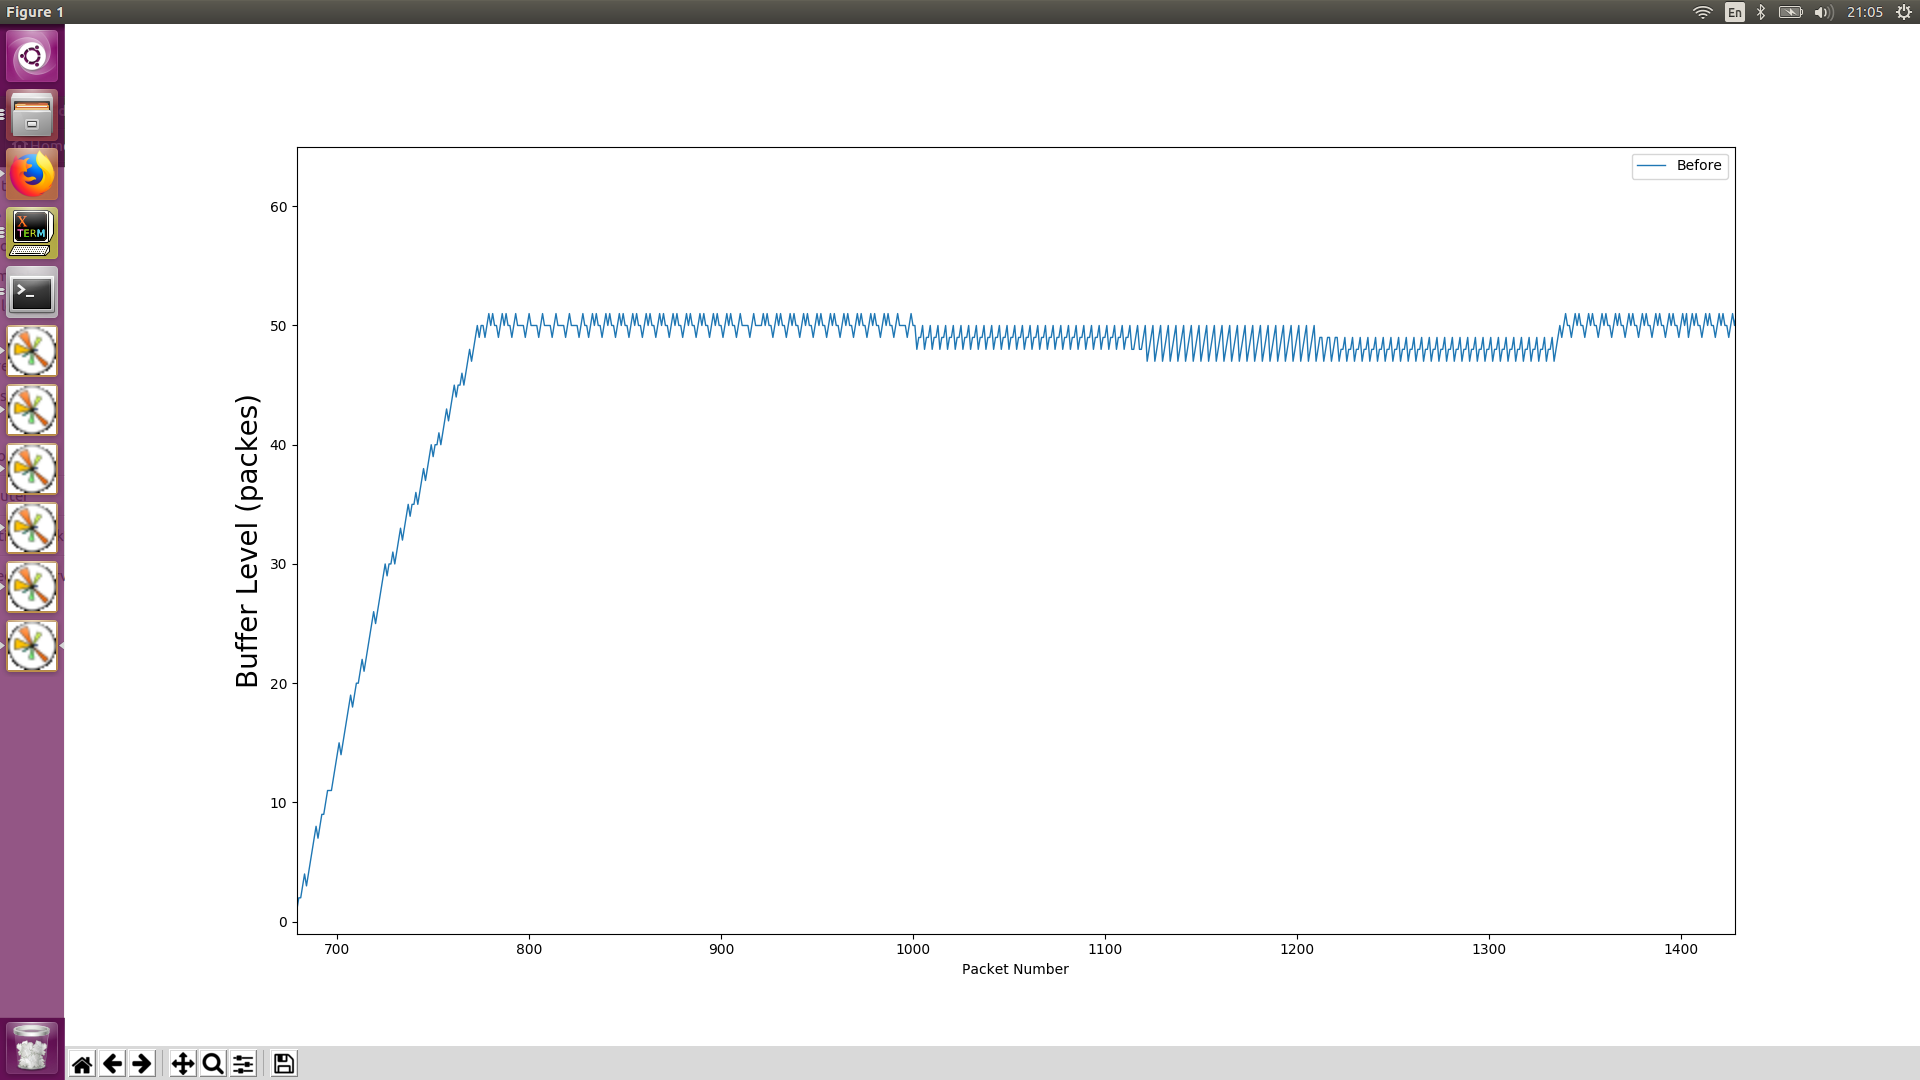
\includegraphics[width=\textwidth]{fig/tail_scenario1_buffer.png}
    %%%% figure needs to be changed %%%%%
	\caption{Buffer level of tail logic in scenario 1}
	\label{tail_scenario1_buffer} 
	\end{minipage}
	\hfill\begin{minipage}[t]{0.23\textwidth}
	\centering
	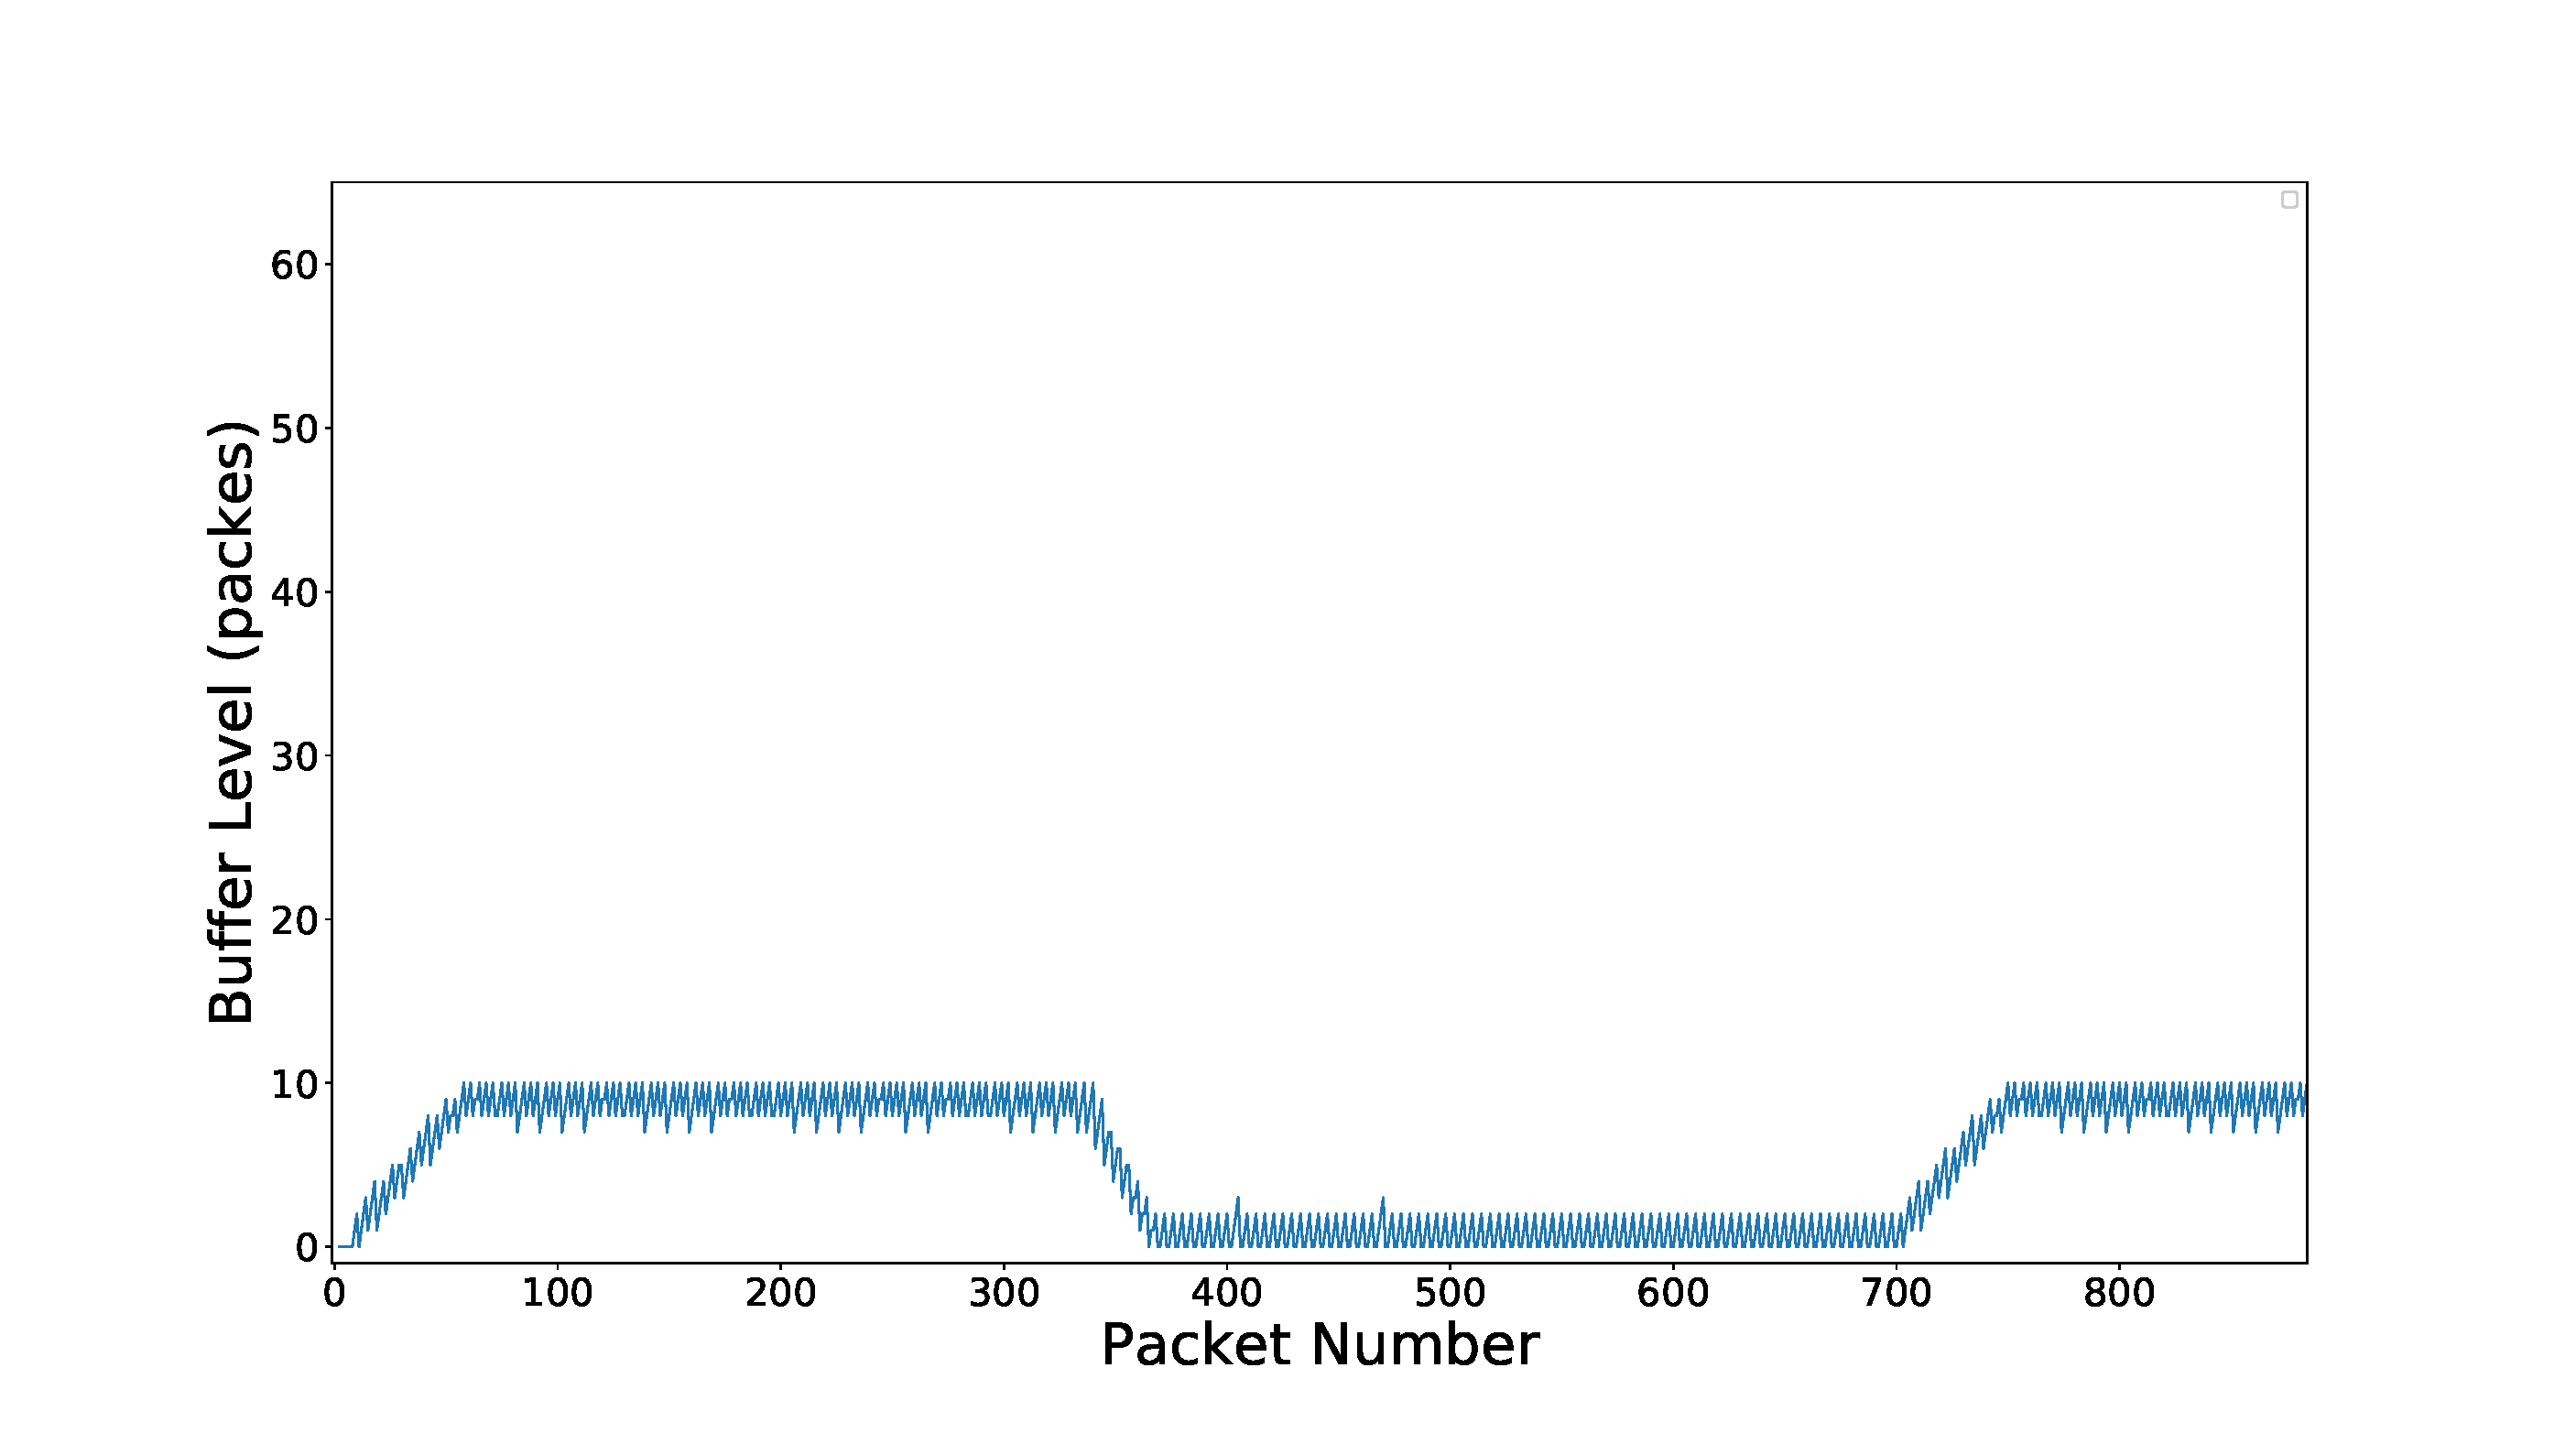
\includegraphics[width=\textwidth]{fig/EL_scenario1_buffer.eps}
	\caption{Buffer level of tail logic in scenario 1}
	\label{EL_scenario1_buffer} 
	\end{minipage}
	\vspace{-0.1cm}
\end{figure}

Despite of the result of received packets. We also plot the buffer level of each experiment. In these figures, x-axis represents the packets count and y-axis represents the quantities of packets inside the queue. We can observe that the buffer level of tail logic in scenario 1 in Fig.~\ref{tail_scenario1_buffer} grows up in the beginning and stop at 85\%, the threshold we set, and continue to the end of streaming. This is because we start to drop everything coming into our MANE.

Fig.~\ref{EL_scenario1_buffer} shows the buffer level of EL logic in scenario 1. We can observe that the buffer level also grows up in the beginning. However, it starts to drop some packets when the buffer level exceeds our threshold. In this scenario, the first threshold let MANE drops enough packets to maintain the buffer level. Then we raise the packet process rate of MANE, and buffer level goes down. Finally, it raise again because we reduce the packet process rate.
\end{subsection}
%%%%% change the figures %%%%%

\begin{subsection}{Scenario 2}

\begin{figure}[tbh]
	\centering
	\begin{minipage}[t]{0.24\textwidth}
	\centering
	\includegraphics[width=\textwidth]{fig/tail_received_packets.eps}
	\caption{Result of Tail Logic in Scenario 2. (Flow 1)}
	\label{tail_received_packets_S2_V1} 
	\end{minipage}
	\hfill\begin{minipage}[t]{0.23\textwidth}
	\centering
	\includegraphics[width=\textwidth]{fig/EL_received_packets.eps}
	\caption{Result of tail Logic in Scenario 2. (Flow 2)}
	\label{tail_received_packets_S2_V2} 
	\end{minipage}
	\vspace{-0.1cm}
\end{figure}

\begin{figure}[tbh]
	\centering
	\begin{minipage}[t]{0.24\textwidth}
	\centering
	\includegraphics[width=\textwidth]{fig/tail_received_packets.eps}
	\caption{Result of EL Logic in Scenario 2. (Flow 1)}
	\label{el_received_packets_S2_V1} 
	\end{minipage}
	\hfill\begin{minipage}[t]{0.23\textwidth}
	\centering
	\includegraphics[width=\textwidth]{fig/EL_received_packets.eps}
	\caption{Result of EL Logic in Scenario 2. (Flow 2)}
	\label{EL_received_packets_S2_V2} 
	\end{minipage}
	\vspace{-0.1cm}
\end{figure}

%%%%%

Fig.~\ref{tail_received_packets_S2_V1} and~\ref{tail_received_packets_S2_V2} shows the result of two streaming flows in scenario 2. Due to the characteristic of bmv2, we can use twice of buffer compare to scenario 1. Therefore we are actually doing the same thing as scenario 1 but do it twice. We can see that the result of flow 1 and flow 2 are almost the same. However, the tail logic sometimes performs very good or very bad. We assume it's because one of the flow occupy the network bandwidth so the other flow could not even get into the MANE or it arrives after the buffer level exceeds the threshold and leads to packet drop. In EL logic, we can see that results are also very similar. However, this result is much more stable. Even we run this experiment many times, the result doesn't change much. Since we have twice of the egress buffer, the result of the buffer level is also similar to scenario 1. Through this scenario, we can know how P4 specifies bmv2 to process packets and prove that using two buffers doesn't affect the efficiency of bmv2.

\end{subsection}

\begin{subsection}{Scenario 3}
    In Scenario 3, we stream two videos in the same buffer. Therefore, the results could be much worse than other scenarios. However, we still want to see the difference between tail and EL logics. Hence, we can observe if there are two video stream in the same buffer, how could RDO choose to stream.

    \begin{figure}[tbh]
        \centering
        \begin{minipage}[t]{0.24\textwidth}
        \centering
        \includegraphics[width=\textwidth]{fig/RDO_CREW.eps}
        \caption{Result of RDO Logic in Scenario 3. (Flow 1)}
        \label{RDO_received_packets_S3_V1} 
        \end{minipage}
        \hfill\begin{minipage}[t]{0.23\textwidth}
        \centering
        \includegraphics[width=\textwidth]{fig/RDO_ICE.eps}
        \caption{Result of RDO Logic in Scenario 3. (Flow 2)}
        \label{RDO_received_packets_S3_V2} 
        \end{minipage}
        \vspace{-0.1cm}
    \end{figure}

    In RDO logic, we want to maximize the total PSNR value of all video streams. This may lead to a unbalanced packet processing. In extreme examples, some videos provides little quality but cost much bandwidth. Therefore, RDO logic aims to choose the video packet provides higher quality and costs less bandwidth. To remark the result, we choose two videos one consists of many moving subject and another has many stable frames. We can see the results in Fig.~\ref{RDO_received_packets_S3_V1} and ~\ref{RDO_received_packets_S3_V2}. 

    Receiver of flow 1 receives 3.17 layers in average and flow 2 receives 2.81. Moreover, the average PSNR value are 33.17db and 29.33db \em{which means the quality is actually twice better than another.} The total average PSNR is ?? which is ?? higher compare to EL logic.

    %%%% change figures %%%%
    \begin{figure}[tbh]
        \centering
        \begin{minipage}[t]{0.24\textwidth}
        \centering
        \includegraphics[width=\textwidth]{fig/RDO_CREW.eps}
        \caption{Result of tail Logic in Scenario 3. (Flow 1)}
        \label{tail_received_packets_S3_V1} 
        \end{minipage}
        \hfill\begin{minipage}[t]{0.23\textwidth}
        \centering
        \includegraphics[width=\textwidth]{fig/RDO_ICE.eps}
        \caption{Result of EL Logic in Scenario 3. (Flow 1)}
        \label{EL_received_packets_S3_V1} 
        \end{minipage}
        \vspace{-0.1cm}
    \end{figure}

    \begin{figure}[tbh]
        \centering
        \begin{minipage}[t]{0.24\textwidth}
        \centering
        \includegraphics[width=\textwidth]{fig/RDO_CREW.eps}
        \caption{Result of EL Logic in Scenario 3. (Flow 2)}
        \label{EL_received_packets_S3_V2} 
        \end{minipage}
        \hfill\begin{minipage}[t]{0.23\textwidth}
        \centering
        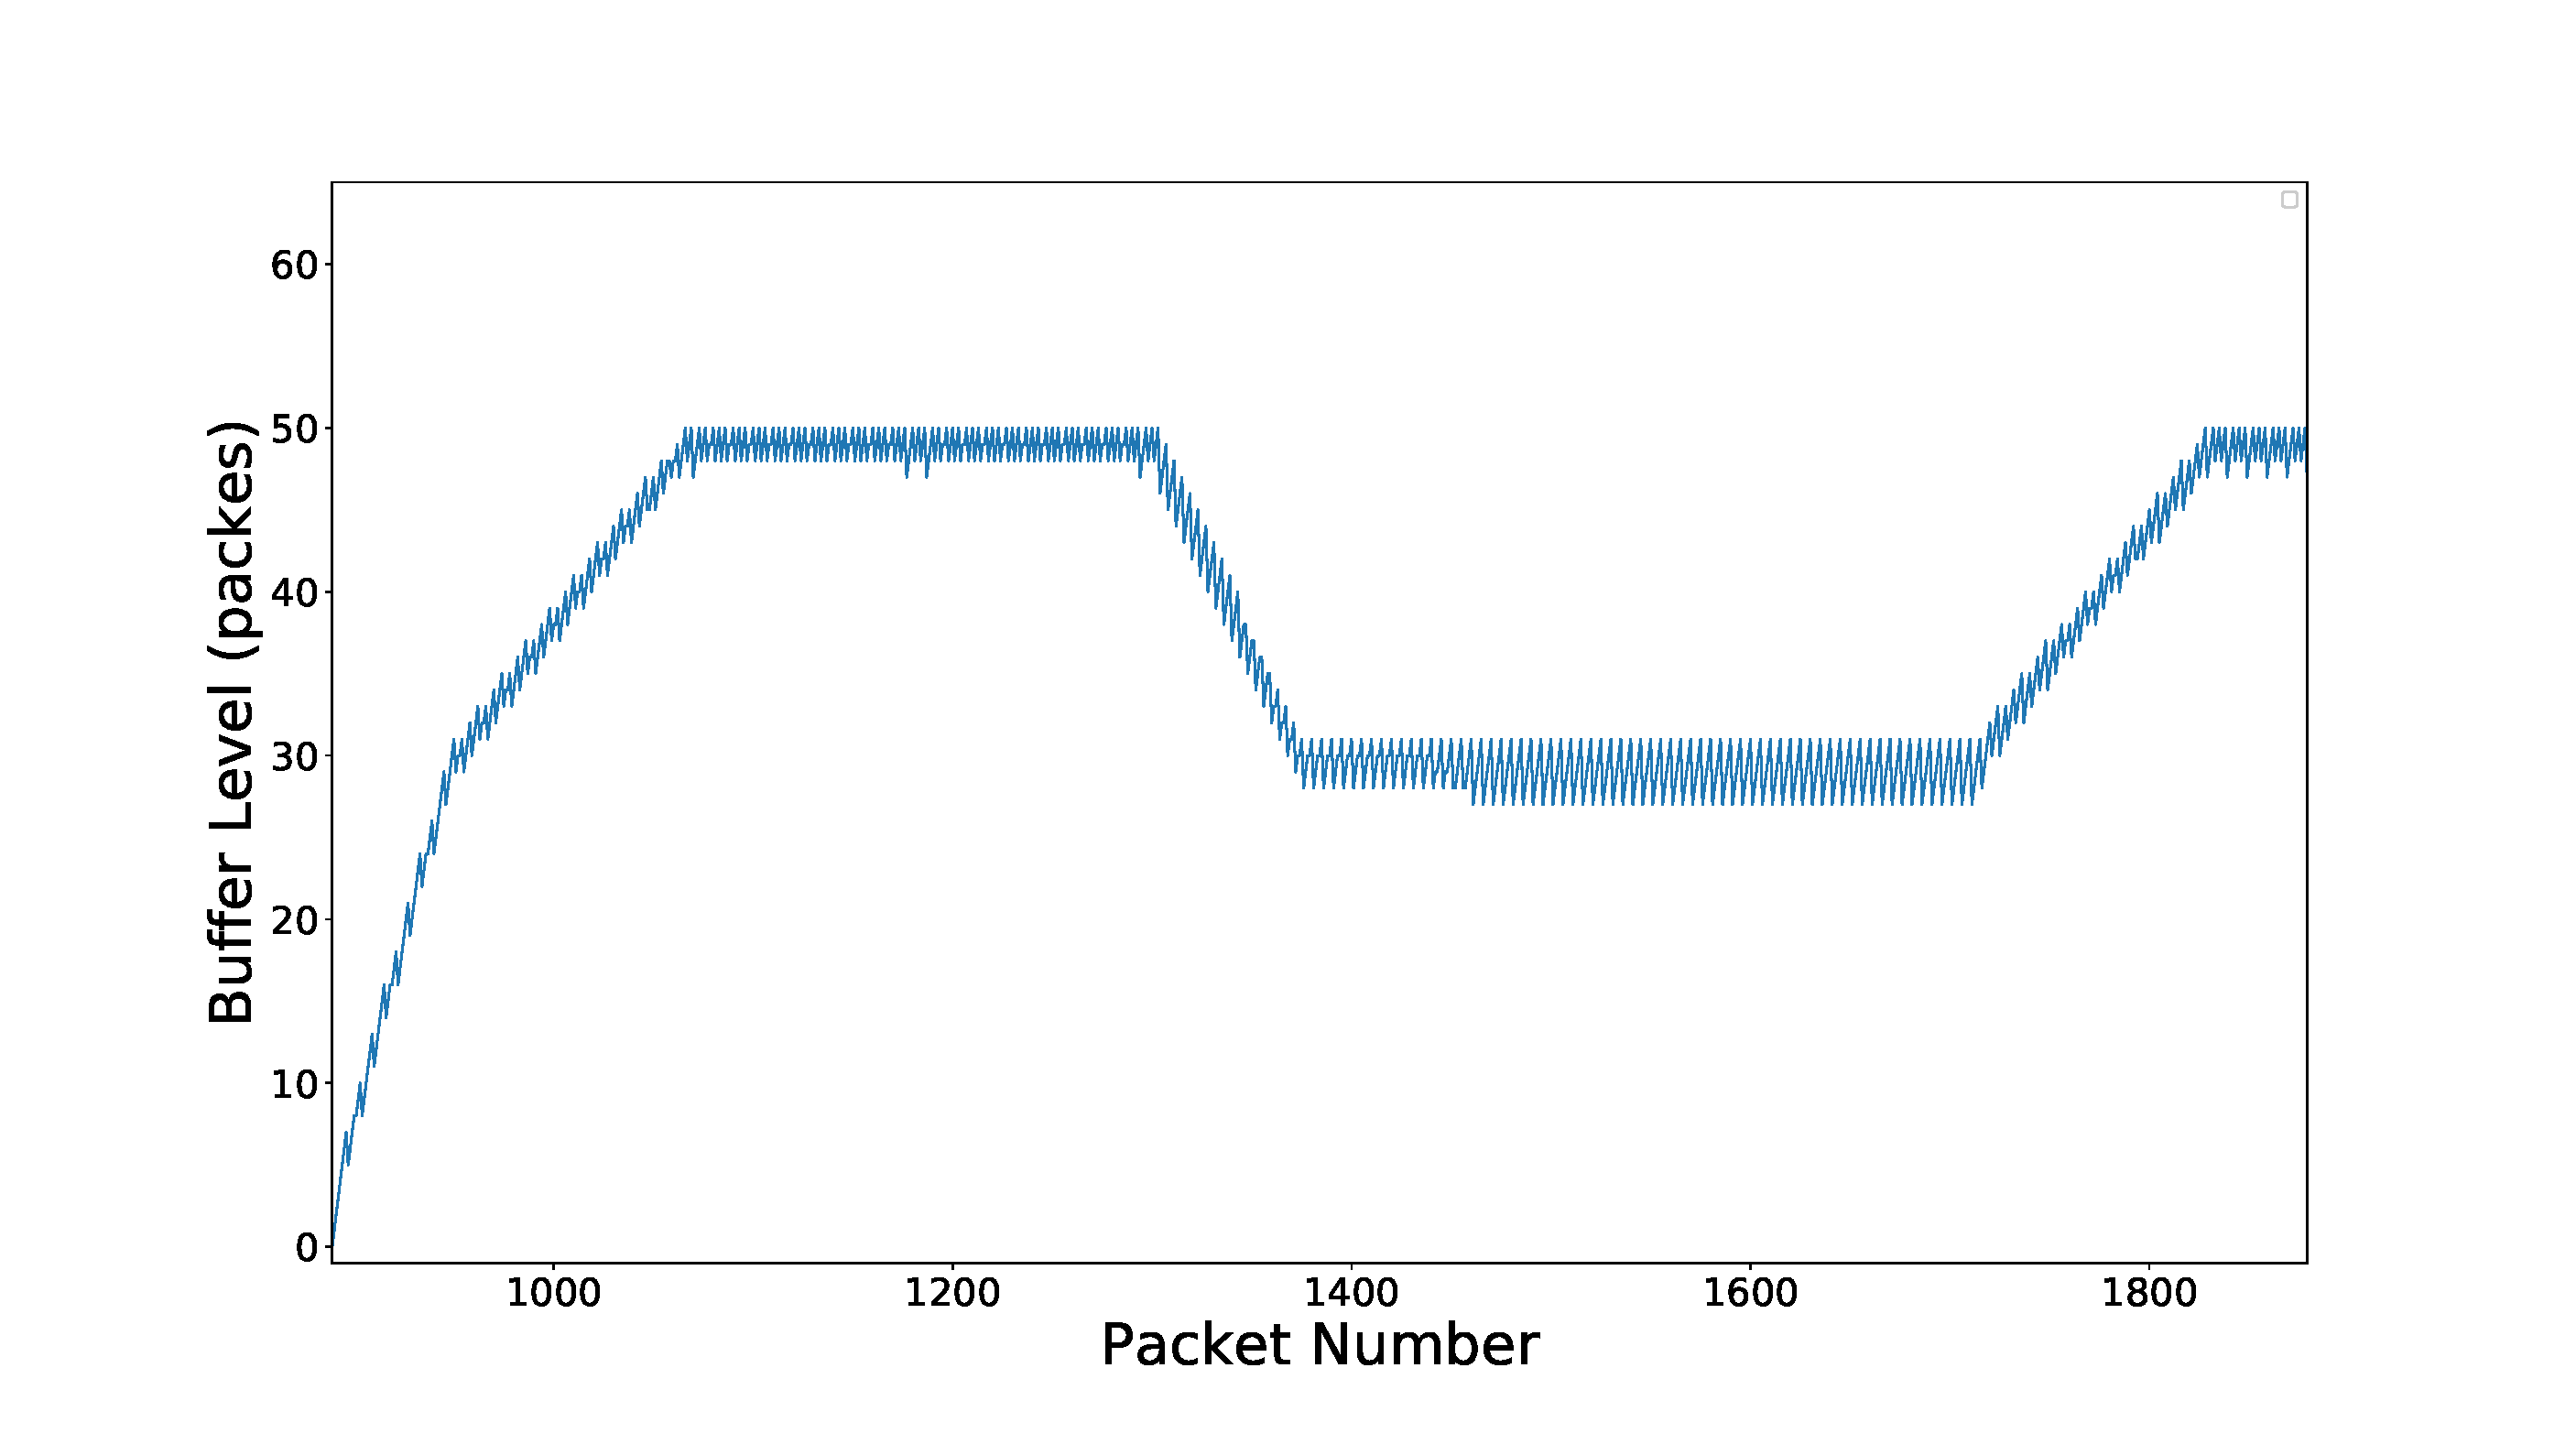
\includegraphics[width=\textwidth]{fig/EL_scenario3_buffer.eps}
        \caption{Buffer level of EL Logic in Scenario 3. (Flow 2)}
        \label{EL_buffer_level_S3_V2} 
        \end{minipage}
        \vspace{-0.1cm}
    \end{figure}
    %%%%


\end{subsection}